\documentclass[11pt]{IEEEtran}
\IEEEoverridecommandlockouts
% The preceding line is only needed to identify funding in the first footnote. If that is unneeded, please comment it out.
\usepackage{cite}
\usepackage{amsmath,amssymb,amsfonts}
\usepackage{algorithmic}
\usepackage{graphicx}
\usepackage{textcomp}
\def\BibTeX{{\rm B\kern-.05em{\sc i\kern-.025em b}\kern-.08em
    T\kern-.1667em\lower.7ex\hbox{E}\kern-.125emX}}
    
\graphicspath{ {figs/} }
\begin{document}

\title{Visualization Dashboard for Rigidity Analysis of Protein Mutations}

\author{\IEEEauthorblockN{Dylan Carpenter, Josh Dombal, Hunter Read}\\
\IEEEauthorblockA{\textit{Western Washington University} \\
Bellingham, WA, USA}
}

\maketitle

\begin{abstract}
Analyzing the effects of protein mutation is crucial to future treatments and development of novel medications for some diseases. However wet lab experiments can be time consuming and exhaustive screenings of protein mutations impossible. To this end, several tools, and computational software can guide this research, but may not provide overall insights into all possible protein mutations. For this, we have developed a visualization dashboard that enables easier insights into the effects of protein mutation through rigidity analysis, and is an effective tool in exploration and identification of possible critical mutations. We conclude that our visualization dashboard allows for novel insight into exhaustive protein mutation data.\\
\end{abstract}

\begin{IEEEkeywords}
bioinformatics, mutation, protein, rigidity, visualization
\end{IEEEkeywords}

\section{Introduction}
Gaining insight into protein mutations is important for researchers and pharmaceutical companies looking to develop new treatments and medications. With some insight into mutant proteins, we could advance cancer diagnosis, prognosis, and therapies \cite{b2}, develop novel medications for Fabry disease, or further a general understanding into many illnesses that plague civilization. Current techniques allow experimentalist to mutate and analyze these variations in a wet lab, but can require months of work with only the hope of providing the information scientists may need\cite{b3}. But due to these time requirements, thorough and exhaustive protein mutation screenings are difficult for small proteins and impossible for large proteins, arising a need for in-silico protein mutation and analysis.\\

While several computational approaches allow for an exploration of mutant proteins, they are frequently limited to a single mutation at a time.  One technique to understand a mutant protein, would be to view a 3D structure in relation to the wild type. This however is limiting, in that human understanding from a structural visualization is limited, and finding differences between a multitude of mutant proteins is impossible. Other techniques involve exploring protein folding comparatively between the wild type and a mutant protein, but this data can be difficult to interpret when the differences are small \cite{b4}. This also does not allow for some understanding and comparative analysis in regards to an exhaustive mutation screen.\\ 

Our technique combines the novel approach of rigidity analysis, exhaustive in-silico mutation data, and a comparative metric combined into a powerful visualization dashboard to provide a unique and powerful insight into the changes between various mutations. Applying rigidity analysis to a protein allows us to gain insight into the structure of the protein. Since structure is crucial to the function of a protein, this insight can be of remarkable use. Rigidity analysis models the biomolecule as a mechanical structure, by identifying stabilizing interactions, and identifying rigid units. Then from the mechanical model, an associated graph is developed, and an efficient algorithm allows us to infer the rigid and flexible regions of this graph. This approach does not require costly energy calculations as is required by some other techniques, or require large datasets as is necessary for machine learning methods. Rigidity analysis allows for insight into protein stability, flexibility, and chemical clustering that may guide a deeper understanding for further exploration in a wet lab environment.\\

For this work, we have gathered computed rigidity analysis data for six proteins of various sizes and provide an interactive dashboard that allows for the exploration of mutations in regards to the wild type and comparatively for the exhaustive mutation screening.



\section{Methods}
\subsection{Data}\label{AA}
The data collected is the result of output from KINARI \cite{b1}, which provides the rigidity analysis data consisting of cluster sizes and the counts of each cluster size as seen in Figure \ref{fig:rigidityAnalysis}. The output of KINARI also provides information about average cluster size, degrees of freedom, and other mechanical model information. KINARI processes the data for the wild type natively, but requires additional software to handle mutations. ProMuteHT \cite{b5} provides the compute pipeline for generating mutants and SCWRL4 \cite{b6} allows for side-chain conformations to larger residues using homology modeling. With this combination of tools, the data has been generated for an exhaustive set of every possible amino acid substitution in a given protein.\\

However, the generated data is raw, unprocessed, and distributed among countless files. This proves rather difficult to interpret and analyze the results. The raw data files are collected together and the valuable data is extracted from the output files. Using the cluster size and count metrics, we then compute a rigidity distance metric, which compares the wild type distributions to each mutation, given by the equation $RD_{WT \rightarrow mutant} : \sum_{i=1}^{LRC} i \times [WT_i - Mut_i]$. This metric can provide some intuition about the protein's stability, with negative rigidity distance being a more unstable mutation, and a positive rigidity distance, more stable. All the data is gathered into a single json file for a protein and provides the foundation for the visualizations.

\begin{figure}[ht]
  \center
  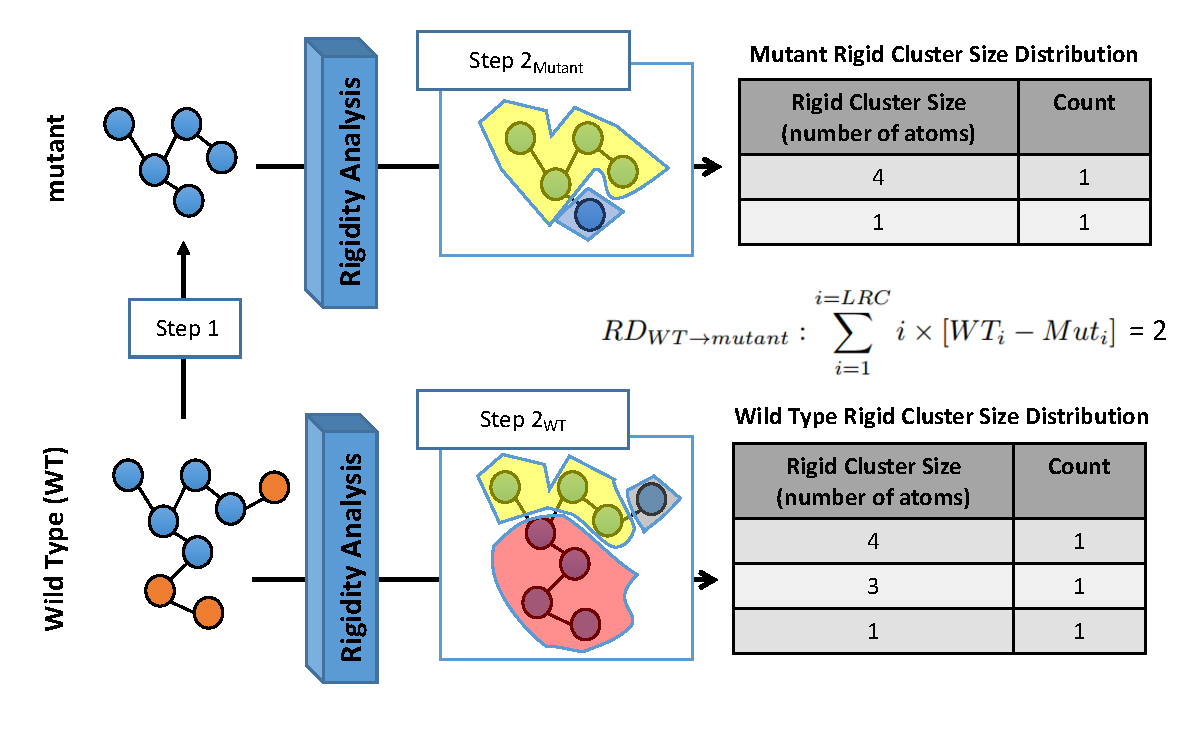
\includegraphics[width=0.45\textwidth]{figs/rigidityCompare.pdf}
  \caption{Rididity Analysis provides insight into cluster size and cluster counts for proteins. Rigidity distance can be calculated from this information with the equation given.}
  \label{fig:rigidityAnalysis}
\end{figure}
\subsection{Visualization Tools}\label{AA}
The overall dashboard was constructed using html, css, and some simple javascript. This contains the header bar that allows for protein selection and heatmap options menu. All tools were built using web frameworks which allows for an easily deployable web application, and powerful extensibility with other web frameworks for further improvements.\\

The heatmap was built entirely using the version 3 of the framework D3 \cite{b7}. First, we process the json data used for only for the heatmap into a 2-dimensional array of objects. This array provides the foundation of the heatmap, with the object at each index containing the values for rigidity distance, cluster information, and the mechanical model information of the mutant. The array is arranged in such a way that the columns represent the amino acid that was substituted in place of the wild type's residue, and the rows represent the numbered amino acid in the chain that makes up the protein. Of note is amino acid's that would not be mutated, as they would represent no substitution of amino acid from the wild type, which have no object values at the given index.\\ 

Then using D3, each array element is given a cell in a 2-dimensional svg grid and color scaled to the appropriate values. When a user wishes to change the heatmap options to represent a different subset of data other than rigidity distance, the heatmap transitions to the new data type within the objects at each index. This allows for quick transitions without reloading the entire data set aided by the powerful transition animations from D3. Both the scale and colors update to reflect the new values during the transition, so the user experience is kept fluid and robust. D3 also provides the interactivity necessary for integrating the bar chart, updating the heatmap row and column reductions, and the tooltip information.\\

We used Billboard.js explicitly for the creation of the barchart. First I'll discuss how we accessed and processed our data. The original data came from a json file, but it was processed by D3 before we touched it with Billboard.js. When the data is handed off to us, it is in the form of an object that contains three arrays(mutation, sizes, counts) and each of those contains embedded arrays as well. Every time a mutation is clicked in the hashmap, that data structure is updated appropriately.\\

In order to use that data to create a clustered bar chart, we transform it into a matrix. The challenge here was that every time a new mutation was added, we had to create a new matrix and fill in empty values with 0 as the number of mutations grew. To create the matrix, we used nested hashmaps to map mutations to their corresponding sizes and counts. Then while iterating through the matrix, we looked up values in the hashmaps and inserted values accordingly.\\

Once the data was neatly formatted as a matrix, we fed that into Billboard.js and created barchart. We used .generate to create the chart, and within that call we were able to customize our barchart by using different keywords. We sized it, specified our data, the type of chart, size of the bars, x and y labels and formatting.

\section{Visualizations}
A key element to all the visualizations is the protein selection header bar as can be seen in Figure \ref{fig:navbar}. This allows a user to select the from a list of available proteins and investigate each one further. This list is easily extensible when more protein mutation data has been gathered.
\begin{figure}[ht]
  \center
  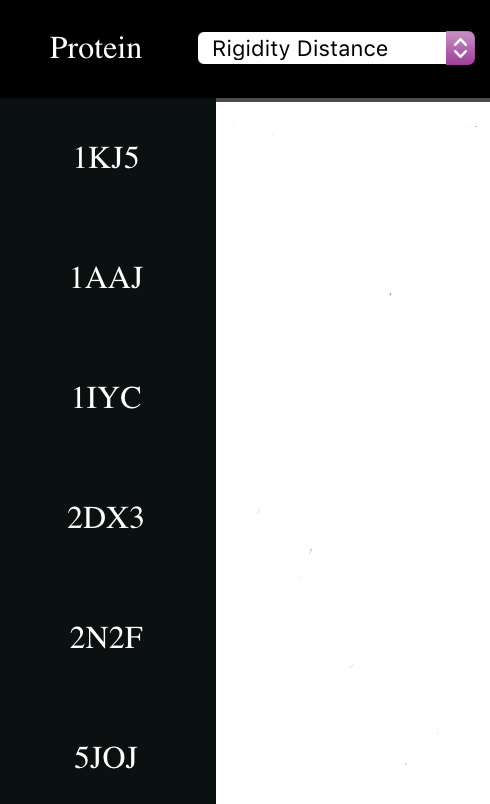
\includegraphics[width=0.15\textwidth]{figs/navbar.png}
  \caption{Protein selection and heatmap data options in fixed navigation bar at the top of the page.}
  \label{fig:navbar}
\end{figure}
\subsection{Heatmap}\label{AA}
We have created a dynamic interactive heatmap that allows for powerful exploration of protein rigidity analysis data. This visualization is the natural choice in support of the data we have. As amino acid and sequence information can be treated as categorical data that can be easily arranged as the indexes for a two dimensional array, which allows the use of area as marks.  With the rigidity distance and other metrics as either diverging or sequential quantitive data, color is used as a channel to show variations in the quantitative attribute.\\

\begin{figure}[ht]
  \center
  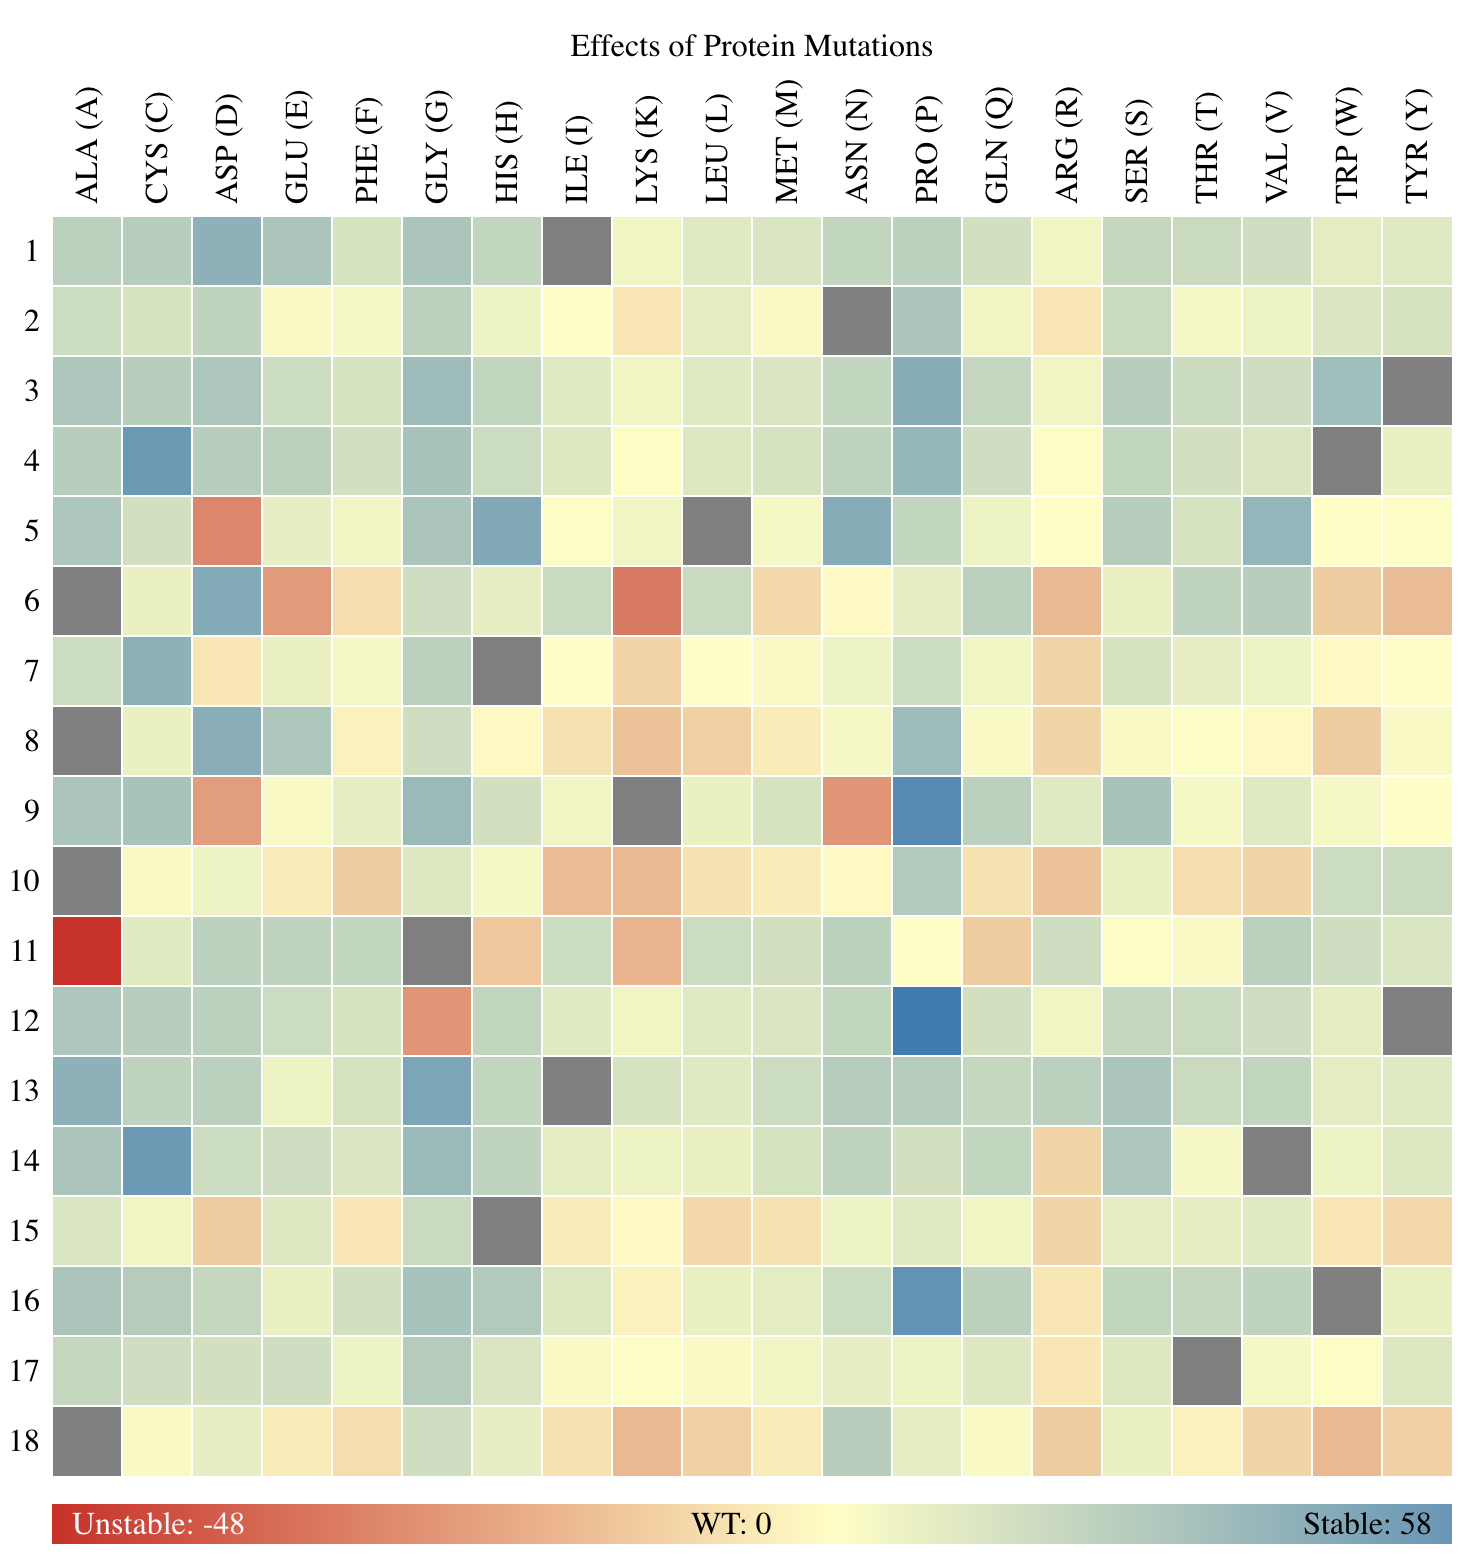
\includegraphics[width=0.45\textwidth]{figs/heatmap_full.png}
  \caption{Heatmap of rigidity distance data for the protein 2DX3}
  \label{fig:heatmapmain}
\end{figure}

Figure \ref{fig:heatmapmain} shows the results of rigidity analysis on protein 2DX3. This view clearly enables a quick view that allows easy identification of an amino acid in sequence and the mutant substitution that was analyzed. This allows for quick identification of outliers, which as can be seen in Figure \ref{fig:heatmapmain}, one mutation has a much larger destabilizing effect than all the other mutant substitutions. Some trends may also be noticeable, as mutations to lysine trend toward a destabilizing effect and mutations to proline have a more frequent stabilizing effect on this protein. \\

Several interactive features are available to enable further exploration of the rigidity analysis data. Figure \ref{fig:heatmapoptions}  shows an options menu that enables different data about cluster distribution, mechanical model differences, and rigidity metrics. This menu is located in the navigation bar, and scrolls with the page so a user can change data without the need to navigate to the top of the page and lose focus on the critical section of the protein they may want to investigate. The heatmap will animate the transition without any interruption to the user experience.\\
\begin{figure}[ht]
  \center
  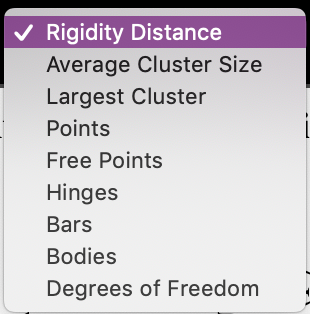
\includegraphics[width=0.15\textwidth]{figs/heatmap_options.png}
  \caption{Heatmap data options in fixed navigation bar at the top of the page.}
  \label{fig:heatmapoptions}
\end{figure}

Figure \ref{fig:heatmapseq} shows a heatmap with degrees of freedom. Some data such as this is treated as sequential data, as the deviation from the wild type is less insightful than for other metrics such as rigidity distance. The wild type information is located in the legend bar below, so that some comparative relation can be inferred if so desired.\\
\begin{figure}[ht]
  \center
  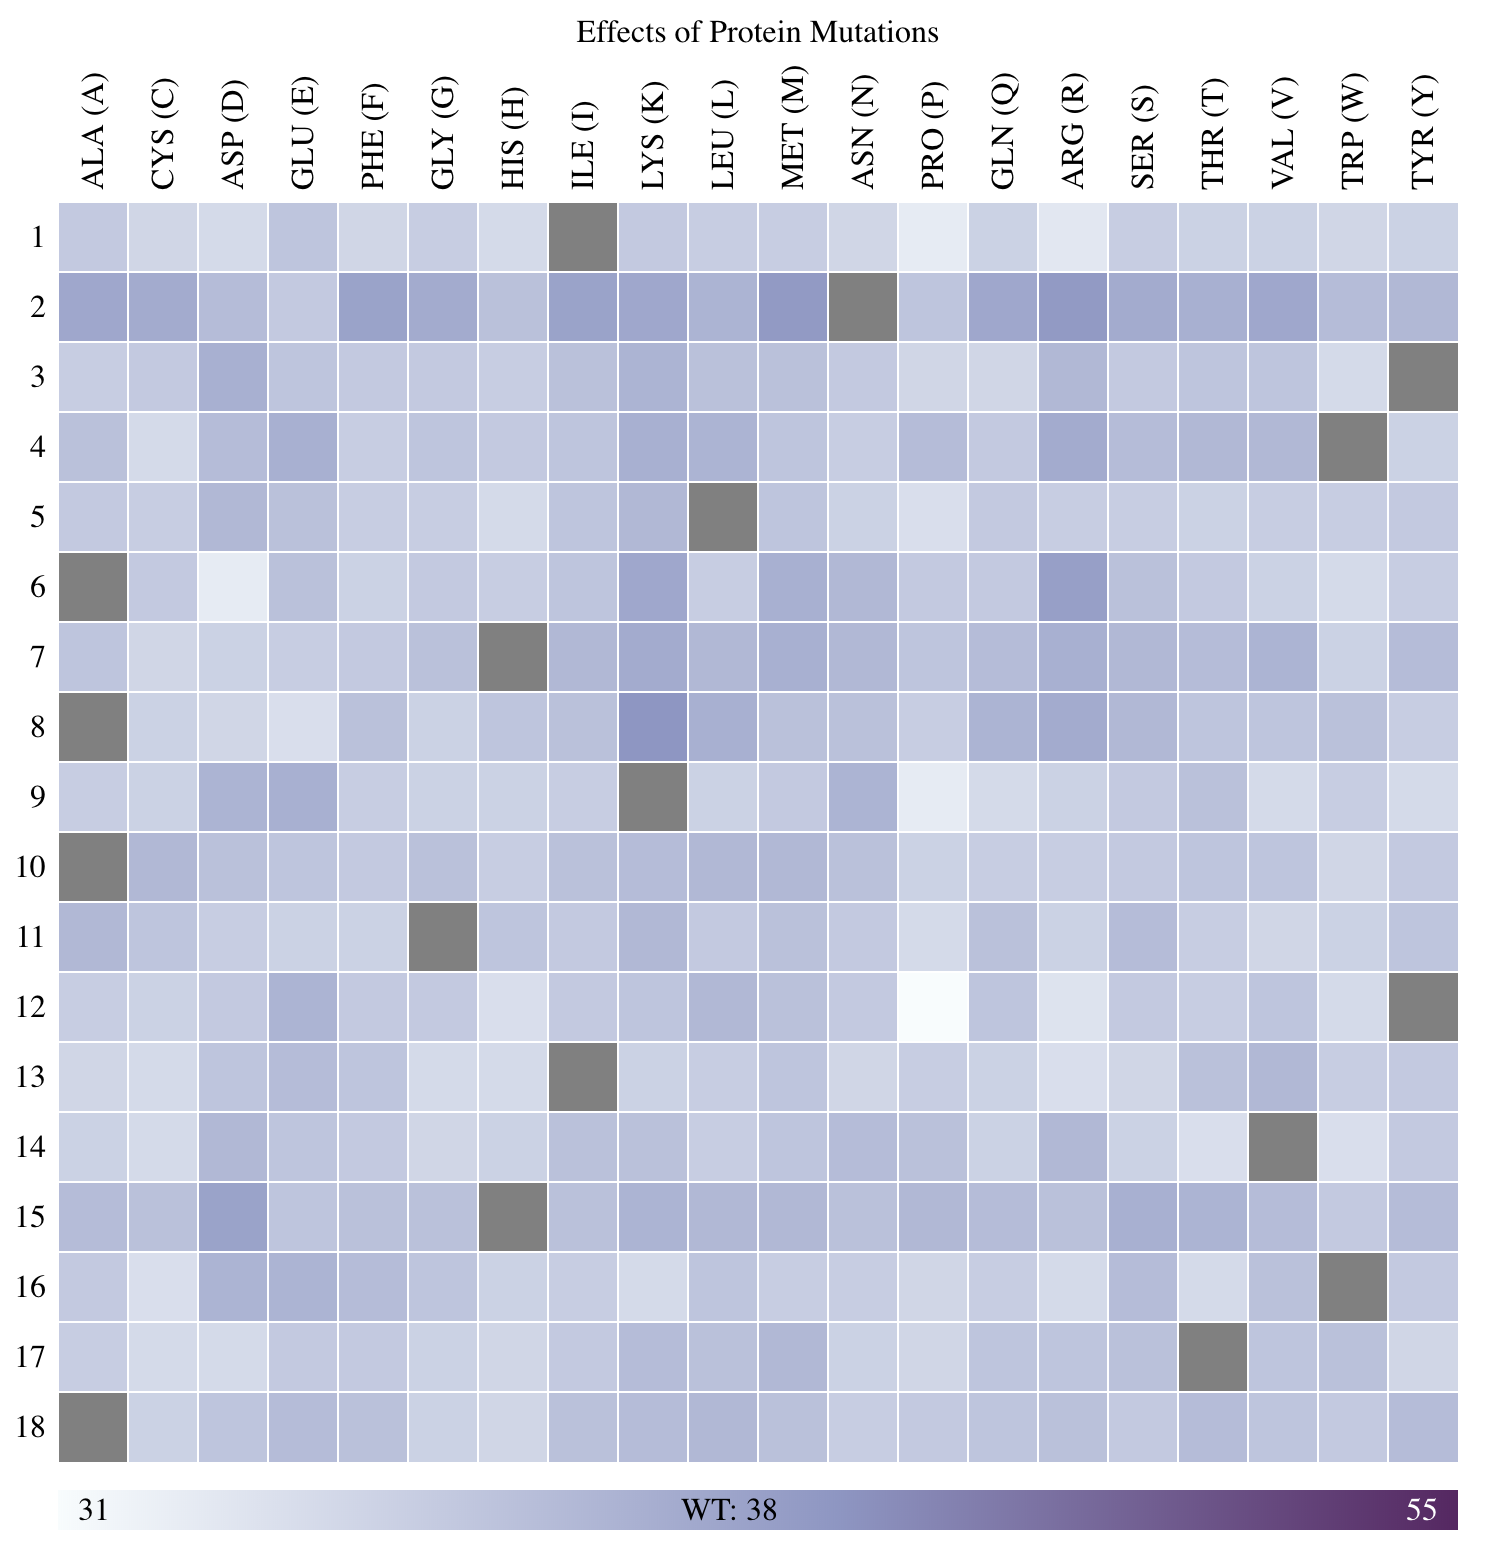
\includegraphics[width=0.45\textwidth]{figs/heatmap_sequential.png}
  \caption{Heatmap of 2DX3 showing degrees of freedom as sequential data.}
  \label{fig:heatmapseq}
\end{figure}

Figure \ref{fig:heatmaptooltip} shows a tooltip that provides more detailed information upon hovering any cell in the heatmap. The rigidity distance is always shown, with the tooltip also including the data for the selected option from Figure \ref{fig:heatmapoptions}.
\begin{figure}[ht]
  \center
  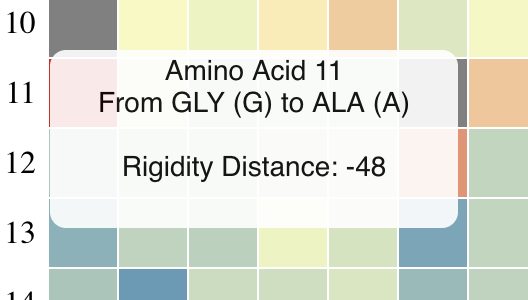
\includegraphics[width=0.35\textwidth]{figs/heatmap_tooltip.png}
  \caption{Tooltip showing detailed information of current mutation on hover of cell}
  \label{fig:heatmaptooltip}
\end{figure}

The heatmap also allows for data reduction, which enable the removal of some outlier data, which con provide even more insights. Clicking any row or column label will remove the selected row or column from the visualization as can be seen in Figure \ref{fig:heatmapreduced}. This allows for a unique comparative assessment when exploring subsequences of the protein data, or an easy method to remove rows or columns that may have an outsized impact and reduce easy identification of other outlying data points. The legend and color range adjust automatically to accommodate the new ranges of values. \\
\begin{figure}[ht]
  \center
  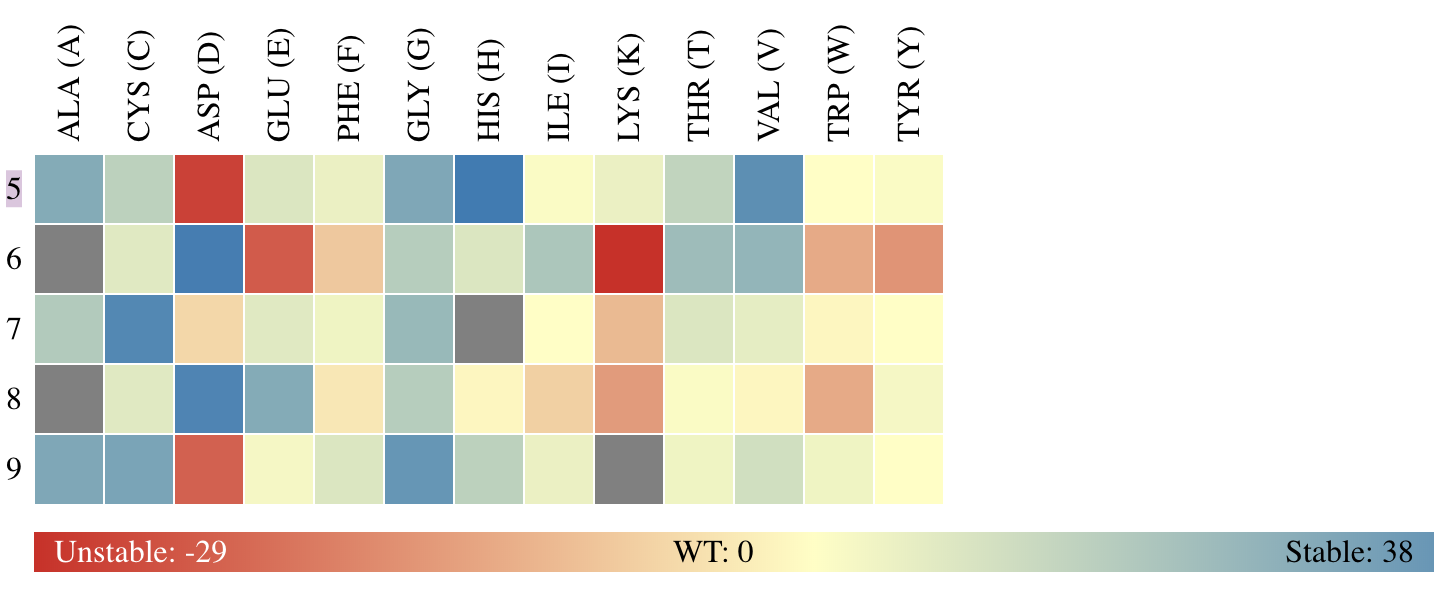
\includegraphics[width=0.45\textwidth]{figs/heatmap_reduced.png}
  \caption{Heatmap of 2DX3 with several rows and columns removed to enable smaller comparative analysis of data}
  \label{fig:heatmapreduced}
\end{figure}

A final feature of the heatmap enables an integration with the bar chart, that when clicking on any cell within the heatmap adds the cluster distribution data to the bar chart for further exploration. 


\subsection{Bar Chart}\label{AA}
We created a dynamic clustered barchart that was designed to accomplish the high level task of analysis. The goal of creating the barchart was to allow the users to consume existing information in order to draw conclusions. The existing data in our project are the counts of specific sizes of clusters in a particular mutation. These mutations can be dynamically chosen from the heatmap, and are then compared with the wild type. After selecting the specific mutations the user wants to compare, they can then come to conclusions or new hypotheses more easily by being able to compare differences side by side. \\

The marks that are used are vertical bars; which represent the different sizes of clusters in the chart. We used multiple channels when designing our barchart. We used position on a common sale because it is very effective to compare different values. We also used color hue so that the user can easily identify the different mutations on the chart simply by looking at the colors. We also made use of horizontal position in order to separate the different sizes of clusters. We used multiple channels so that the user can easily look at the chart from different angles and analyze the chart for different purposes.\\ 

Figure ???? shows the basic chart before any mutations have been added from the heatmap.


\section{Findings}


\section{Discussion}

\section{Conclusions}



%\cite{b1}

\begin{thebibliography}{00}
\bibitem{b1} N. Fox, F. Jagodzinski, and I. Streinu. "Kinari-lib: a C++ library for pebble game rigidity analysis of mechanical models." In Minisymposium on Publicly Available Geometric/Topological Software, 2012.
\bibitem{b2} Q. Wang, R. Chaerkady, J. Wu, H. Hwang, N. Papadopoulos, L. Kopelovich, et al. "Mutant proteins as cancer-specific biomarkers". Proceedings of the National Academy of Sciences. 2011.
\bibitem{b3} T. Maximova, R. Moatt, B. Ma, R. Nussinov, and A. Shehu. "Principles and overview of sampling methods for modeling macromolecular structure and dynamics." PLoS computational biology. 2016.
\bibitem{b4} A. Oliveira Jr., F. Fatore, F. Paulovich, O. Oliveira Jr., and V. Leite  "Visualization of Protein Folding Funnels in Lattice Models." PLoS computational biology. 2014.
\bibitem{b5} E. Andersson and F. Jagodzinski. "ProMuteHT: A high throughput compute pipeline for generating protein mutants in silico." In Proceedings of the
8th ACM International Conference on Bioinformatics, Computational Biology, and Health Informatics 2017.
\bibitem{b6} G. Krivov, M. Shapovalov, and R. Dunbrack. "Improved prediction of protein side-chain conformations with scwrl4". Proteins: Structure,
Function, and Bioinformatics, 2009.
\bibitem{b7} M. Bostock, V. Ogievetsky, and J. Heer. "D3 Data-Driven Documents". IEEE Transactions on Visualization and Computer Graphics, 2011.	



\end{thebibliography}



\end{document}
